\documentclass[fontsize=12pt,paper=a4,twoside]{scrartcl}

\newcommand{\grad}{\ensuremath{^{\circ}} }
\renewcommand{\strut}{\vrule width 0pt height5mm depth2mm}

\usepackage[utf8]{inputenc}
\usepackage[final]{pdfpages}
% obere Seitenränder gestalten können
\usepackage{fancyhdr}
\usepackage{moreverb}
% Graphiken als jpg, png etc. einbinden können
\usepackage{graphicx}
\usepackage{stmaryrd}
% Floats Objekte mit [H] festsetzen
\usepackage{float}
% setzt URL's schön mit \url{http://bla.laber.com/~mypage}
\usepackage{url}
% Externe PDF's einbinden können
\usepackage{pdflscape}
% Verweise innerhalb des Dokuments schick mit " ... auf Seite ... "
% automatisch versehen. Dazu \vref{labelname} benutzen
\usepackage[ngerman]{varioref}
\usepackage[ngerman]{babel}
\usepackage{ngerman}
% Bibliographie
\usepackage{bibgerm}
% Tabellen
\usepackage{tabularx}
\usepackage{supertabular}
\usepackage[colorlinks=true, pdfstartview=FitV, linkcolor=blue,
            citecolor=blue, urlcolor=blue, hyperfigures=true,
            pdftex=true]{hyperref}
\usepackage{bookmark}

\hyphenation{Arbeits-paket}

\newboolean{langversion} %Deklaration
\setboolean{langversion}{true} %Zuweisung ist 'false' für Blockkurs
\newcommand{\highlight}[1]{\textcolor{blue}{\textbf{#1}}}
\newcommand{\nurlangversion}[0]{%
\ifthenelse{\boolean{langversion}}{\highlight{Muss in SWP-2 ausgefüllt werden}}{\highlight{Entfällt in SWP-1}}}


\newcommand{\swp}[0]{\ifthenelse{\boolean{langversion}}%
{Software--Projekt 2}{Software--Projekt 1}}
\newcommand{\jahr}[0]{2014}
\newcommand{\semester}[0]{\ifthenelse{\boolean{langversion}}{WiSe}{SoSe}}

% erstes Argument: SWP-2, zweites SWP-1
\newcommand{\variante}[2]{\ifthenelse{\boolean{langversion}}{#1}{#2}}

% Damit Latex nicht zu lange Zeilen produziert:
\sloppy
%Uneinheitlicher unterer Seitenrand:
%\raggedbottom

% Kein Erstzeileneinzug beim Absatzanfang
% Sieht aber nur gut aus, wenn man zwischen Absätzen viel Platz einbaut
\setlength{\parindent}{0ex}

% Abstand zwischen zwei Absätzen
\setlength{\parskip}{1ex}

% Seitenränder für Korrekturen verändern
\addtolength{\evensidemargin}{-1cm}
\addtolength{\oddsidemargin}{1cm}

\bibliographystyle{gerapali}

% Lustige Header auf den Seiten
  \pagestyle{fancy}
  \setlength{\headheight}{70.55003pt}
  \fancyhead{}
  \fancyhead[LO,RE]{\swp\\ \semester \jahr
  \\Architekturbeschreibung}
  \fancyhead[LE,RO]{Seite \thepage\\\slshape \leftmark\\\slshape \rightmark}

%Etwas größere Zeilenabstände in Tabellen
\renewcommand{\arraystretch}{1.2}

%
% Und jetzt geht das Dokument los....
%

\begin{document}

% Lustige Header nur auf dieser Seite
  \thispagestyle{fancy}
  \fancyhead[LO,RE]{ }
  \fancyhead[LE,RO]{Universität Bremen\\FB 3 -- Informatik\\
  Prof. Dr. Rainer Koschke \\TutorIn: Karsten Hölscher}
  \fancyfoot[C]{}

% Start Titelseite
  \vspace{3cm}

  \begin{minipage}[H]{\textwidth}
  \begin{center}
  \bf
  \Large
  Software--Projekt 2 2014\\
  \smallskip
  \small
  VAK 03-BA-901.02\\
  \vspace{3cm}
  \end{center}
  \end{minipage}
  \begin{minipage}[H]{\textwidth}
  \begin{center}
  \vspace{1cm}
  \bf
  \Large Architekturbeschreibung\\
  \vspace{3ex}
   	  \begin{figure}[H]
      \centering
      
\includegraphics[width=0.25\textwidth]{../WOYM.png}
      \end{figure}
  \vfill
  \end{center}
  \end{minipage}
  \vfill
  \begin{minipage}[H]{\textwidth}
  \begin{center}
  \sf
  \begin{tabular}{l}
  Tim Hansen \\
  Joshua Hoffmann\\
  Hassan Klait \\
  Adrian Lück \\
  Jurij Schmidt\\
  Falko Schröder
  \end{tabular}
  \\ ~
  \vspace{2cm}
  \\
  \it Version 1.0\\ ~
  \end{center}
  \end{minipage}

% Ende Titelseite

% Start Leerseite

\newpage

  \thispagestyle{fancy}
  \fancyhead{}
  \fancyhead[LO,RE]{\swp{} \\  \semester{} \jahr{}
  \\Architekturbeschreibung}
  \fancyhead[LE,RO]{Seite \thepage\\\slshape \leftmark\\~}
  \fancyfoot{}
  \renewcommand{\headrulewidth}{0.4pt}
  \tableofcontents

\newpage

  \fancyhead[LE,RO]{Seite \thepage\\\slshape \leftmark\\\slshape \rightmark}


%%%%%%%%%%%%%%%%%%%%%%%%%%%%%%%%%%%%%%%%%%%%%%%%%%%%%%%%%%%%%%%%%%%%%%%%
\section*{Version und Änderungsgeschichte}

\begin{tabular}{ccl}
Version & Datum & Änderungen \\
\hline
1.0 & 29.10.2014 & Dokumentvorlage als initiale Fassung kopiert  \\
1.1 & 22.11.2014 & Erste vollständige Fassung der konzeptionellen und Datensicht\\
\end{tabular}


%%%%%%%%%%%%%%%%%%%%%%%%%%%%%%%%%%%%%%%%%%%%%%%%%%%%%%%%%%%%%%%%%%%%%%%%
\section{Einführung}

\subsection{Zweck}
  
Die Architekturbeschreibung soll es anderen Entwicklern ermöglichen, den Aufbau der Software und Intentionen hinter bestimmten Design-Entscheidungen zu verstehen. Dadurch sollen Fremdentwickler in die Lage versetzt werden, die Software zu überarbeiten und Bugs zu beheben.

\subsection{Status}
\nurlangversion


  
\subsection{Definitionen, Akronyme und Abkürzungen}


\subsection{Referenzen}
Die folgenden Kapitel stützen sich im Wesentlichen auf die Vorlesungsfolien ,,Software-Architektur 1`` der Veranstaltung ,,Software-Projekt 1`` im Sommersemester 2014 an der Universität Bremen von Prof. Dr. Rainer Koschke.


\subsection{Übersicht über das Dokument}
\nurlangversion


\section{Globale Analyse}
\label{sec:globale_analyse}

\subsection{Einflussfaktoren}
\label{sec:einflussfaktoren}
{\it Hier sind Einflussfaktoren gefragt, die sich auf die Architektur
  beziehen. Es sind ausschließlich architekturrelevante
  Einflussfaktoren, und nicht z.B.\ solche, die lediglich einen
  Einfluss auf das Projektmanagement haben. Fragt Euch also bei jedem
  Faktor: Beeinflusst er wirklich die Architektur? Macht einen
  einfachen Test: Wie würde die Architektur aussehen, wenn ihr den
  Einflussfaktor E berücksichtigt? Wie würde sie aussehen, wenn Ihr E nicht
  berücksichtigt? Kommt in beiden Fällen dieselbe Architektur heraus,
  dann kann der Einflussfaktor nicht architekturrelevant sein.

  Es geht hier um Einflussfaktoren, die
  \begin{enumerate}
  \item sich über die Zeit ändern,
  \item viele Komponenten betreffen,
  \item schwer zu erfüllen sind oder
  \item mit denen man wenig Erfahrung hat.
  \end{enumerate}
  Die Flexibilität und Veränderlichkeit müssen ebenfalls charakterisiert werden. 
  \begin{enumerate}
  \item Flexibilität: Könnt Ihr den Faktor zum jetzigen Zeitpunkt beeinflussen?
  \item Veränderlichkeit: ändert der Faktor sich später durch äußere Einflüsse?
\end{enumerate}

  Unter Auswirkungen sollte dann beschrieben werden, {\em wie} der
  Faktor {\em was} beeinflusst. Das können sein:
  \begin{itemize}
  \item andere Faktoren
  \item Komponenten
  \item Operationsmodi
  \item Designentscheidungen (Strategien)
  \end{itemize}

  Verwendet eine eindeutige Nummerierung der Faktoren, um sie auf den
  Problemkarten einfach referenzieren zu können.  }

\subsubsection{Organisatorische Faktoren}
\begin{tabularx}{\textwidth}{|p{3.5cm}|X|X|}
\hline
\textbf{Faktor} & \textbf{Flexibilität und Veränderlichkeit} & \textbf{Auswirkung}\\\hline
\end{tabularx}\newline

\begin{tabularx}{\textwidth}{|p{3.5cm}|X|X|}
\hline
\multicolumn{3}{|l|}{\textbf{O1: Management}}\\\hline
\multicolumn{3}{|l|}{O1.1: Zeitplan vs. Funktionsumfang}\\\hline
Der Zeitplan ist in jedem Fall einzuhalten. Ggf. muss dafür in Kauf genommen werden, dass gewisse Funktionen fehlen. & Dieser Faktor ist nicht flexibel oder veränderlich. & Nicht alle geplanten Funktionen können implementiert werden. Zunächst Beschränkung auf die Funktionen, die notwendig sind, um die Mindestanforderungen zu erfüllen.\\\hline

\multicolumn{3}{|l|}{\textbf{O2: Personal: Fähigkeiten, Interessen, Stärken, Schwächen}}\\\hline

\multicolumn{3}{|l|}{\textbf{O3: Prozesse und Werkzeuge für die Entwicklungsschritte}}\\\hline

\multicolumn{3}{|l|}{\textbf{O4: Entwicklungszeitplan}}\\\hline

\multicolumn{3}{|l|}{\textbf{O5: Entwicklungsbudget}}\\\hline
\multicolumn{3}{|l|}{O3.1: Anzahl der Entwickler}\\\hline
Es sind maximal sechs Entwickler am Projekt beteiligt. & Es können keine weitere Entwickler hinzugezogen werden. Teilnehmende Entwickler können temporär oder komplett ausfallen. & \\\hline
\end{tabularx}\\

\subsubsection{Technische Faktoren}
\begin{tabularx}{\textwidth}{|p{3.5cm}|X|X|}
\hline
\textbf{Faktor} & \textbf{Flexibilität und Veränderlichkeit} & \textbf{Auswirkung}\\\hline
\end{tabularx}\newline

\begin{tabularx}{\textwidth}{|p{3.5cm}|X|X|}
\hline
\multicolumn{3}{|l|}{\textbf{T1: Hardware}}\\\hline

\multicolumn{3}{|l|}{\textbf{T2: Software}}\\\hline

\multicolumn{3}{|l|}{\textbf{T3: Architekturtechnologie}}\\\hline

\multicolumn{3}{|l|}{\textbf{T4: Standards}}\\\hline
\multicolumn{3}{|l|}{T4.1: Datenbank}\\\hline
Die Verwendung einer leichtgewichtigen, eingebetteten relationalen Datenbank ist vorgeschrieben. & Dieser Faktor ist nicht flexibel oder veränderlich. & \\\hline

\end{tabularx}\\

\subsubsection{Produktfaktoren}
\begin{tabularx}{\textwidth}{|p{3.5cm}|X|X|}
\hline
\textbf{Faktor} & \textbf{Flexibilität und Veränderlichkeit} & \textbf{Auswirkung}\\\hline
\end{tabularx}\newline

\begin{tabularx}{\textwidth}{|p{3.5cm}|X|X|}
\hline
\multicolumn{3}{|l|}{\textbf{P1: Produktfunktionen}}\\\hline

\multicolumn{3}{|l|}{\textbf{P2: Benutzerschnittstelle}}\\\hline

\multicolumn{3}{|l|}{\textbf{P3: Performanz}}\\\hline

\multicolumn{3}{|l|}{\textbf{P4: Verlässlichkeit}}\\\hline

\multicolumn{3}{|l|}{\textbf{P5: Fehlererkennung, -bericht, -behandlung}}\\\hline

\multicolumn{3}{|l|}{\textbf{P6: Service}}\\\hline
\end{tabularx}\\


\subsection{Probleme und Strategien}
\label{sec:strategien}

{\it Aus einer Menge von Faktoren ergeben sich Probleme, die nun in
  Form von Problemkarten beschrieben werden. Diese resultieren
  z.B. aus
  \begin{itemize}
  \item Grenzen oder Einschränkungen durch Faktoren
  \item der Notwendigkeit, die Auswirkung eines Faktors zu begrenzen
  \item der Schwierigkeit, einen Produktfaktor zu erfüllen, oder
  \item der Notwendigkeit einer allgemeinen Lösung zu globalen
    Anforderungen.
  \end{itemize}
  Dazu entwickelt Ihr Strategien, um mit den identifizierten Problemen
  umzugehen.

  Achtet auch hier darauf, dass die Probleme und Strategien wirklich
  die Architektur betreffen und nicht etwa das Projektmanagement. Die
  Strategien stellen im Prinzip die Designentscheidungen dar. Sie
  sollten also die Erklärung für den konkreten Aufbau der
  verschiedenen Sichten liefern.}


\textit{Beschreibt möglichst mehrere Alternativen und gebt
  an, für welche Ihr Euch letztlich aus welchem Grunde entschieden
  habt. Natürlich müssen die genannten Strategien in den folgenden
  Sichten auch tatsächlich umgesetzt werden!}

\textit{Ein sehr häufiger Fehler ist es, dass SWP-Gruppen
  arbeitsteilig vorgehen: die eine Gruppe schreibt das Kapitel zur
  Analyse von Faktoren und zu den Strategien, die andere Gruppe
  beschreibt die diversen Sichten, ohne dass diese beiden Gruppen sich
  abstimmen. Natürlich besteht aber ein Zusammenhang zwischen den
  Faktoren, Strategien und Sichten. Dieser muss erkennbar sein, indem
  sich die verschiedenen Kapitel eindeutig aufeinander beziehen.}

\section{Konzeptionelle Sicht}
\label{sec:konzeptionell}

\begin{figure}[H]
\centering
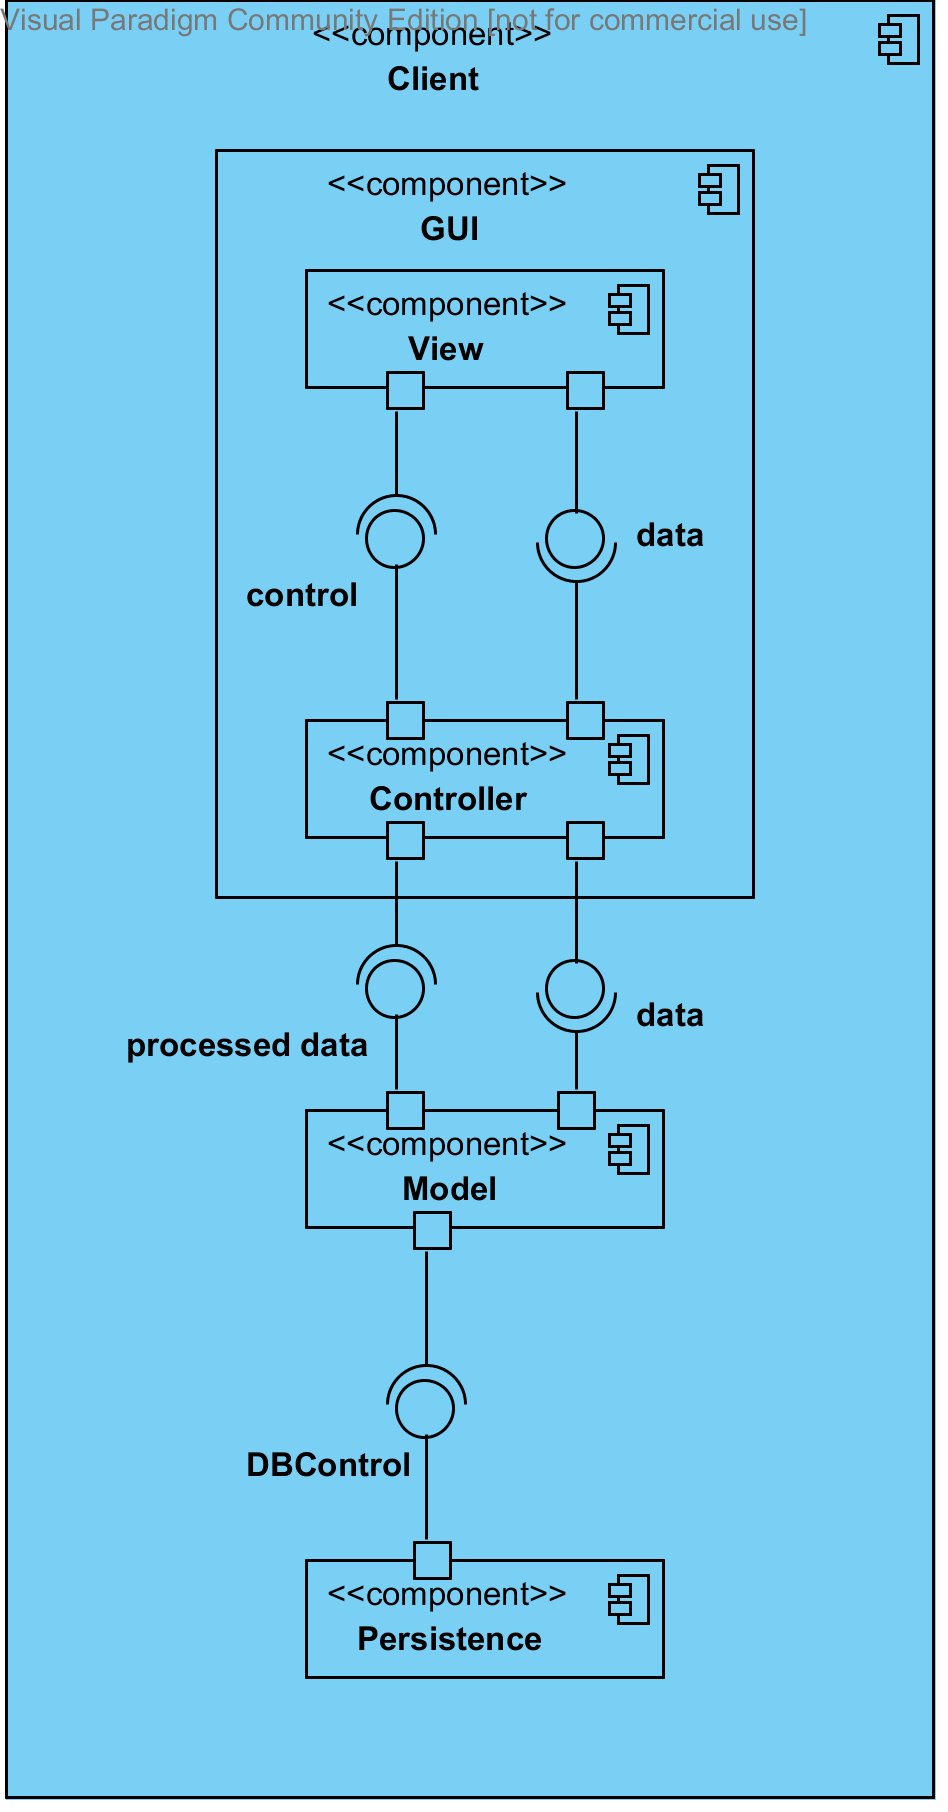
\includegraphics[width=0.35\textwidth]{konzept_sicht.png}
\caption{Konzeptionelle Sicht als UML-Komponentendiagramm}
\end{figure}

Der Client besteht aus der GUI-, Model- und Persistence-Komponente. Die GUI-Komponente ist wiederum unterteilt in View und Controller. Die View-Komponente stellt Daten (in Form von Eingaben des Nutzers) für den Controller bereit. Der Controller hat die Kontrolle über die View-Komponente. Der Controller gibt die von der View-Komponente erhaltenen Daten nach ggf. ersten Validierungen in Form eines Transferobjektes an die Model-Komponenten weiter. Diese implementiert die Logik des Systems. Die Model-Komponente verarbeitet also die erhaltenen Daten, führt ggf. Berechnungen aus und gibt dem Controller in der Regel ein Status-Objekt zurück, welches den Erfolg oder Misserfolg (inkl. Gründen) einer Datenverarbeitung angibt. \\
Auf unterster Ebene befindet sich schließlich die Persistence-Komponente. Diese hat die Kontrolle über die Datenbank und führt dementsprechend die Datenbankanfragen aus. Die Persistence-Komponente wird nur von der Model-Komponente aufgerufen, nicht von der GUI. Die Architektur folgt also dem Schichtenmodell.

\section{Modulsicht}
\label{sec:modulsicht}

{\it
Diese Sicht beschreibt den statischen Aufbau des Systems mit Hilfe von
Modulen, Subsystemen, Schichten und Schnittstellen. 
Diese Sicht ist hierarchisch, d.h. Module werden in Teilmodule
zerlegt. Die Zerlegung endet bei Modulen, die ein klar umrissenes
Arbeitspaket für eine Person darstellen und in einer Kalenderwoche
implementiert werden können. Die Modulbeschreibung der Blätter dieser
Hierarchie muss genau genug und ausreichend sein, um das Modul 
implementieren zu können.

Die Modulsicht wird durch {UML}-Paket- und Klassendiagramme visualisiert.

Die Module werden durch ihre Schnittstellen beschrieben. 
Die Schnittstelle eines Moduls $M$ ist die Menge aller Annahmen, die
andere Module über $M$ machen dürfen, bzw.\ jene Annahmen, die $M$
über seine verwendeten Module macht (bzw. seine Umgebung, wozu auch
Speicher, Laufzeit etc.\ gehören).
Konkrete Implementierungen dieser Schnittstellen sind das Geheimnis des Moduls
und können vom Programmierer festgelegt werden. Sie sollen hier
dementsprechend nicht beschrieben werden. 

Die Diagramme der Modulsicht sollten die zur Schnittstelle gehörenden Methoden
enthalten. Die Beschreibung der einzelnen Methoden (im Sinne der Schnittstellenbeschreibung)
geschieht allerdings per Javadoc im zugehörigen Quelltext. Das bedeutet, dass Ihr
für alle Eure Module Klassen, Interfaces und Pakete erstellt und sie mit den Methoden der
Schnittstellen verseht. Natürlich noch ohne Methodenrümpfe bzw.\ mit minimalen Rümpfen.
Dieses Vorgehen vereinfacht den Schnittstellenentwurf und stellt Konsistenz sicher.

Jeder Schnittstelle liegt ein
Protokoll zugrunde. Das Protokoll beschreibt die Vor- und
Nachbedingungen der Schnittstellenelemente. Dazu gehören die erlaubten
Reihenfolgen, in denen Methoden der Schnittstelle aufgerufen werden
dürfen, sowie Annahmen über Eingabeparameter und Zusicherungen über
Ausgabeparameter. Das Protokoll von Modulen wird in der Modulsicht beschrieben.
Dort, wo es sinnvoll ist, sollte es mit Hilfe von Zustands- oder
Sequenzdiagrammen spezifiziert werden. Diese sind dann einzusetzen, wenn der
Text allein kein ausreichendes Verständnis vermittelt (insbesondere
bei komplexen oder nicht offensichtlichen Zusammenhängen).

Der Bezug zur konzeptionellen Sicht muss klar ersichtlich sein. Im
Zweifel sollte er explizit erklärt werden. Auch für diese Sicht muss
die Entstehung anhand der Strategien erläutert werden.
}

\subsection{Persistenzschicht}

\begin{figure}[H]
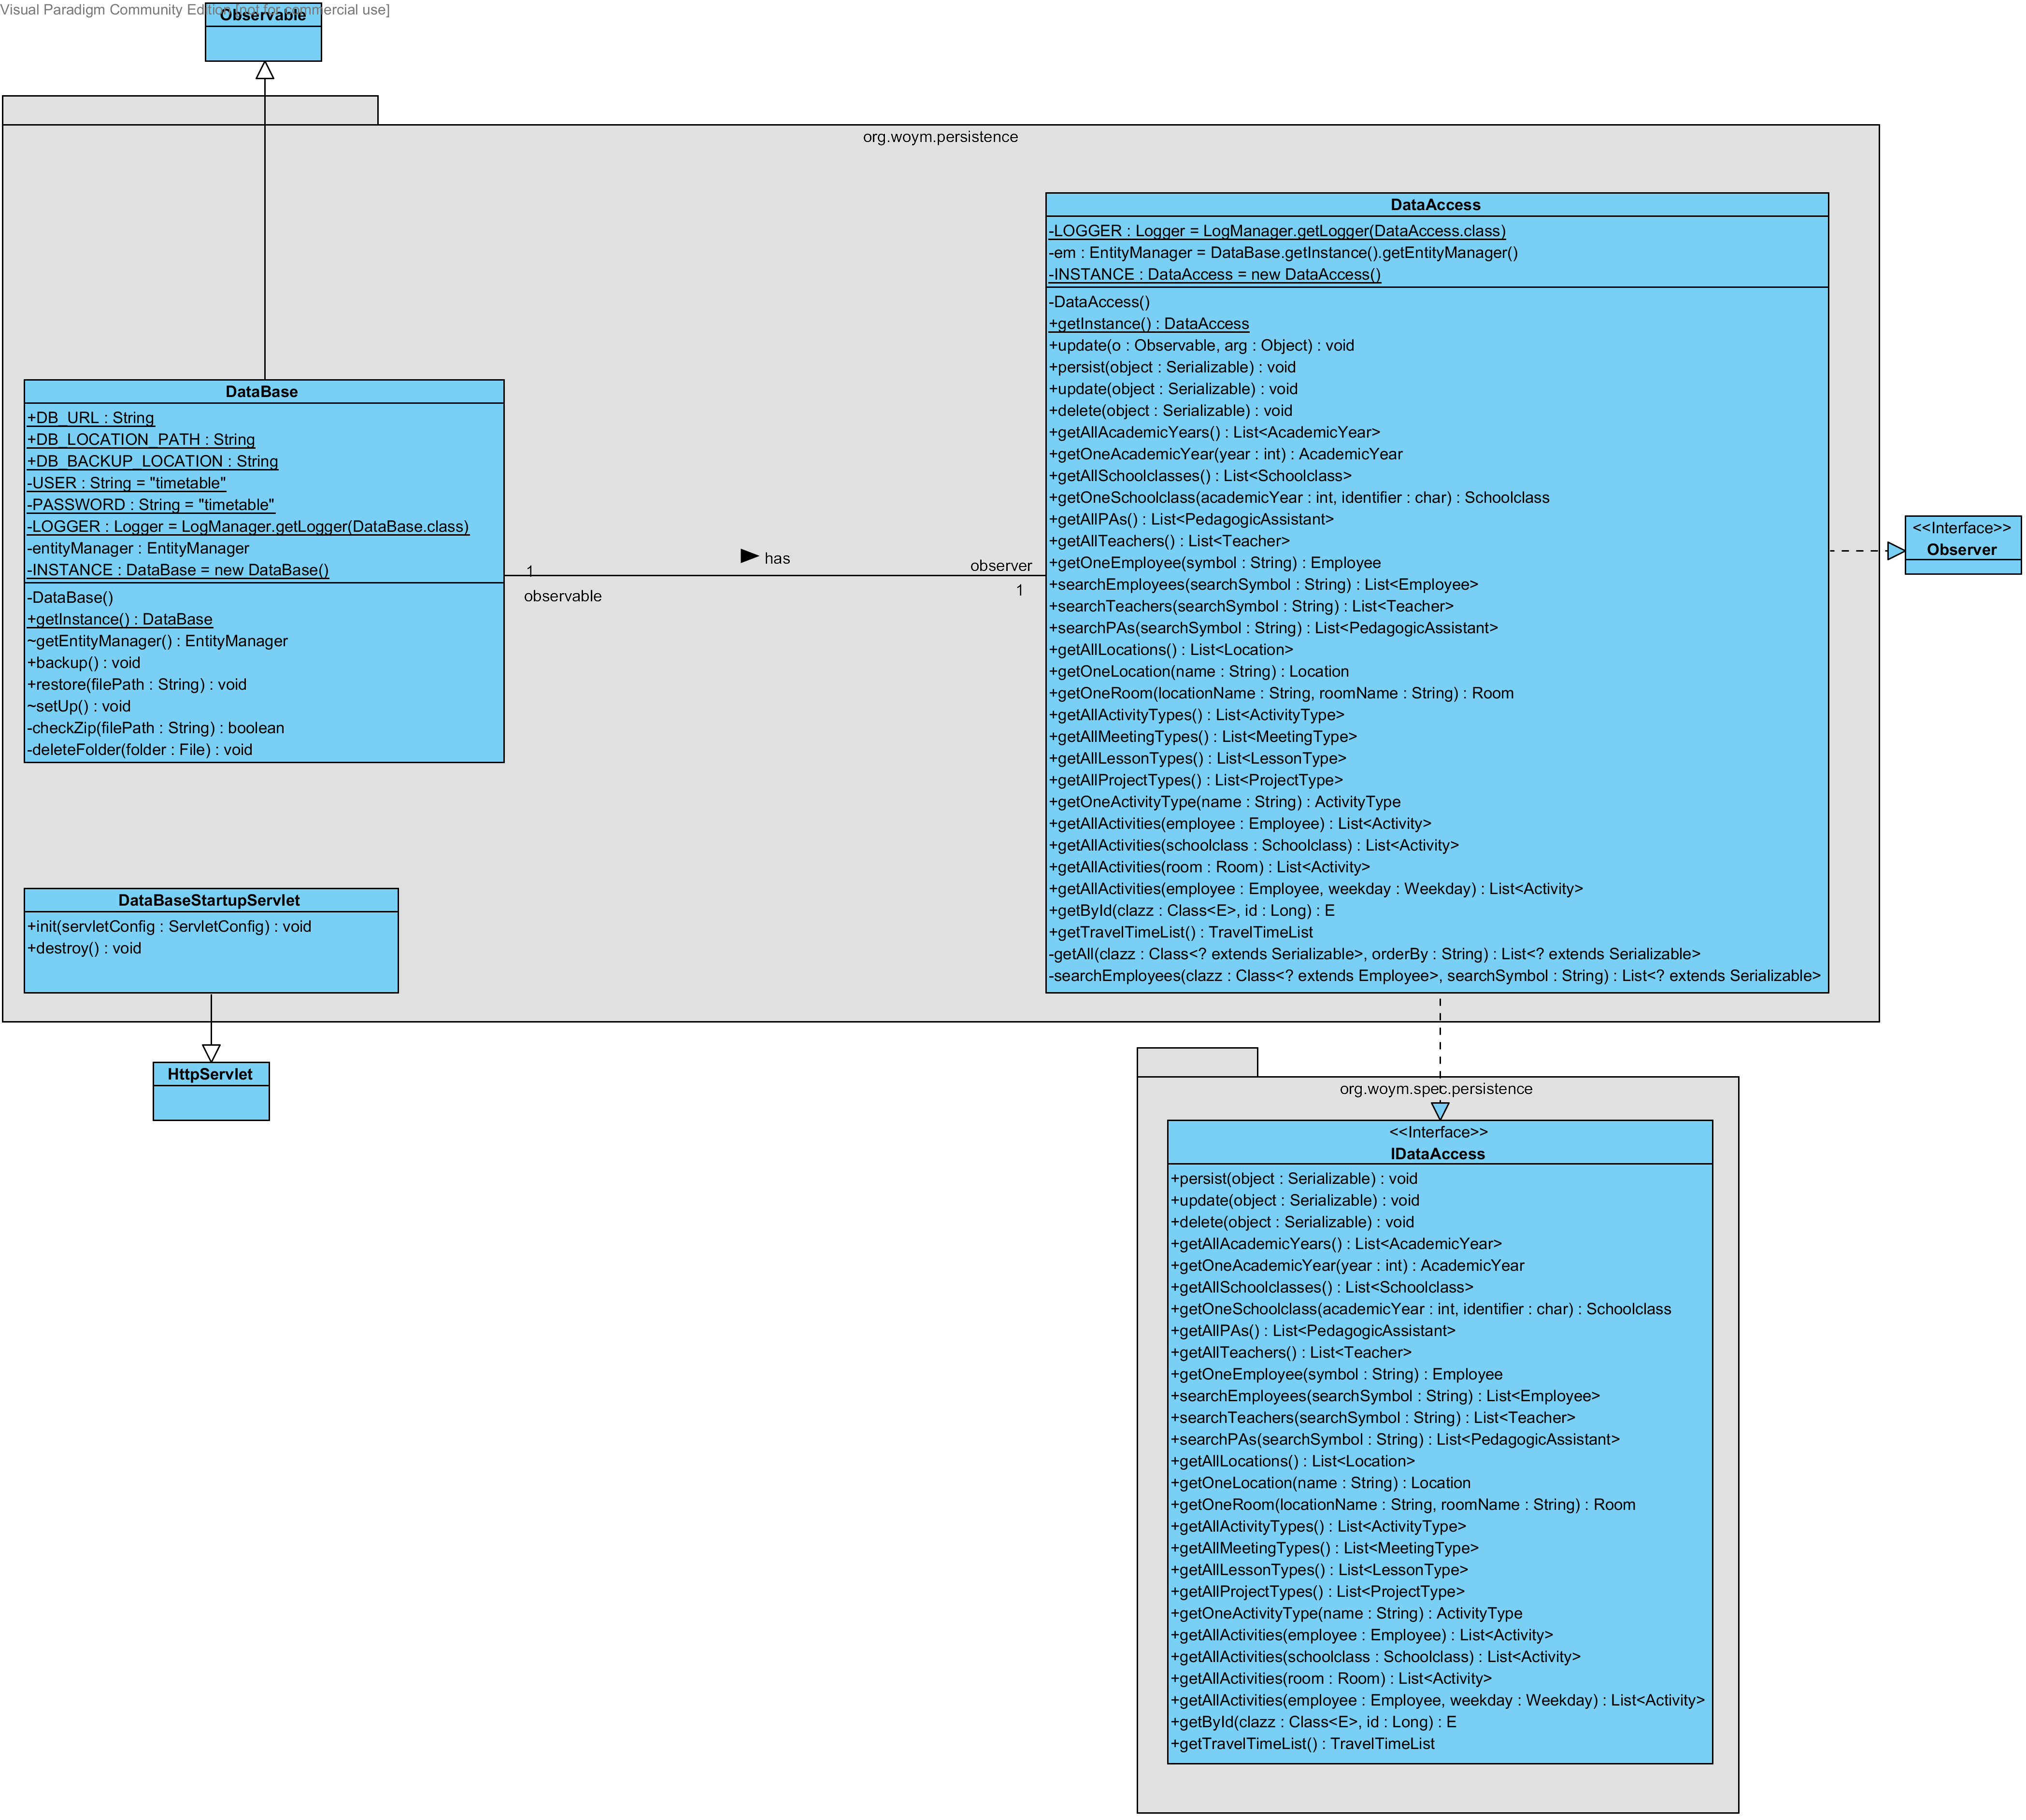
\includegraphics[width=\textwidth]{Persistence.png}
\caption{Klassendiagramm Persistenzschicht}
\end{figure}

Die Persistenzschicht ist für ein Single-User-System konzipiert und besteht aus drei Klassen. Die Singleton-Klasse \texttt{DataBase} stellt die unterste Ebene dar. Dort wird der EntityManager erzeugt, der für alle Datenbankanfragen von \texttt{DataAccess} verwendet wird. Außerdem bietet sie Methoden an, die ein Backup der Datenbank erzeugen bzw. ein Backup wiederherstellen. \texttt{DataBase} erweitert die Java-Klasse \texttt{Observable}, da es für die Wiederherstellung eines Backups notwendig ist, die Datenbank einmal komplett herunterzufahren und danach dementsprechend ein neuer EntityManager verwendet wird. Dies muss den beobachtenden Klassen mitgeteilt werden.\\
Die Singleton-Klasse \texttt{DataAccess} implementiert das Java-Interface \texttt{Observer} und wird bei Erzeugung bei \texttt{DataBase} als Observer registriert. Zudem implementiert sie das Interface \texttt{IDataAccess}, welches alle notwendigen Datenzugriffsmethoden beschreibt. Die Klasse \texttt{DataAccess} stellt also die Schnittstelle zur Datenbank dar.\\
Die letzte Klasse der Persistenzschicht ist \texttt{DataBaseStartupServlet}, welche die Java-Klasse \texttt{HttpServlet} erweitert. Sie dient dazu, die Datenbankverbindung mit dem Hochfahren des Tomcat-Servers aufzubauen. Dazu wird in der \emph{init}-Methode die Methode \emph{setUp} der Klasse \texttt{DataBase} aufgerufen.

\section{Datensicht}
\label{sec:datensicht}
  
\subsection{Datenmodell}

\begin{figure}[H]
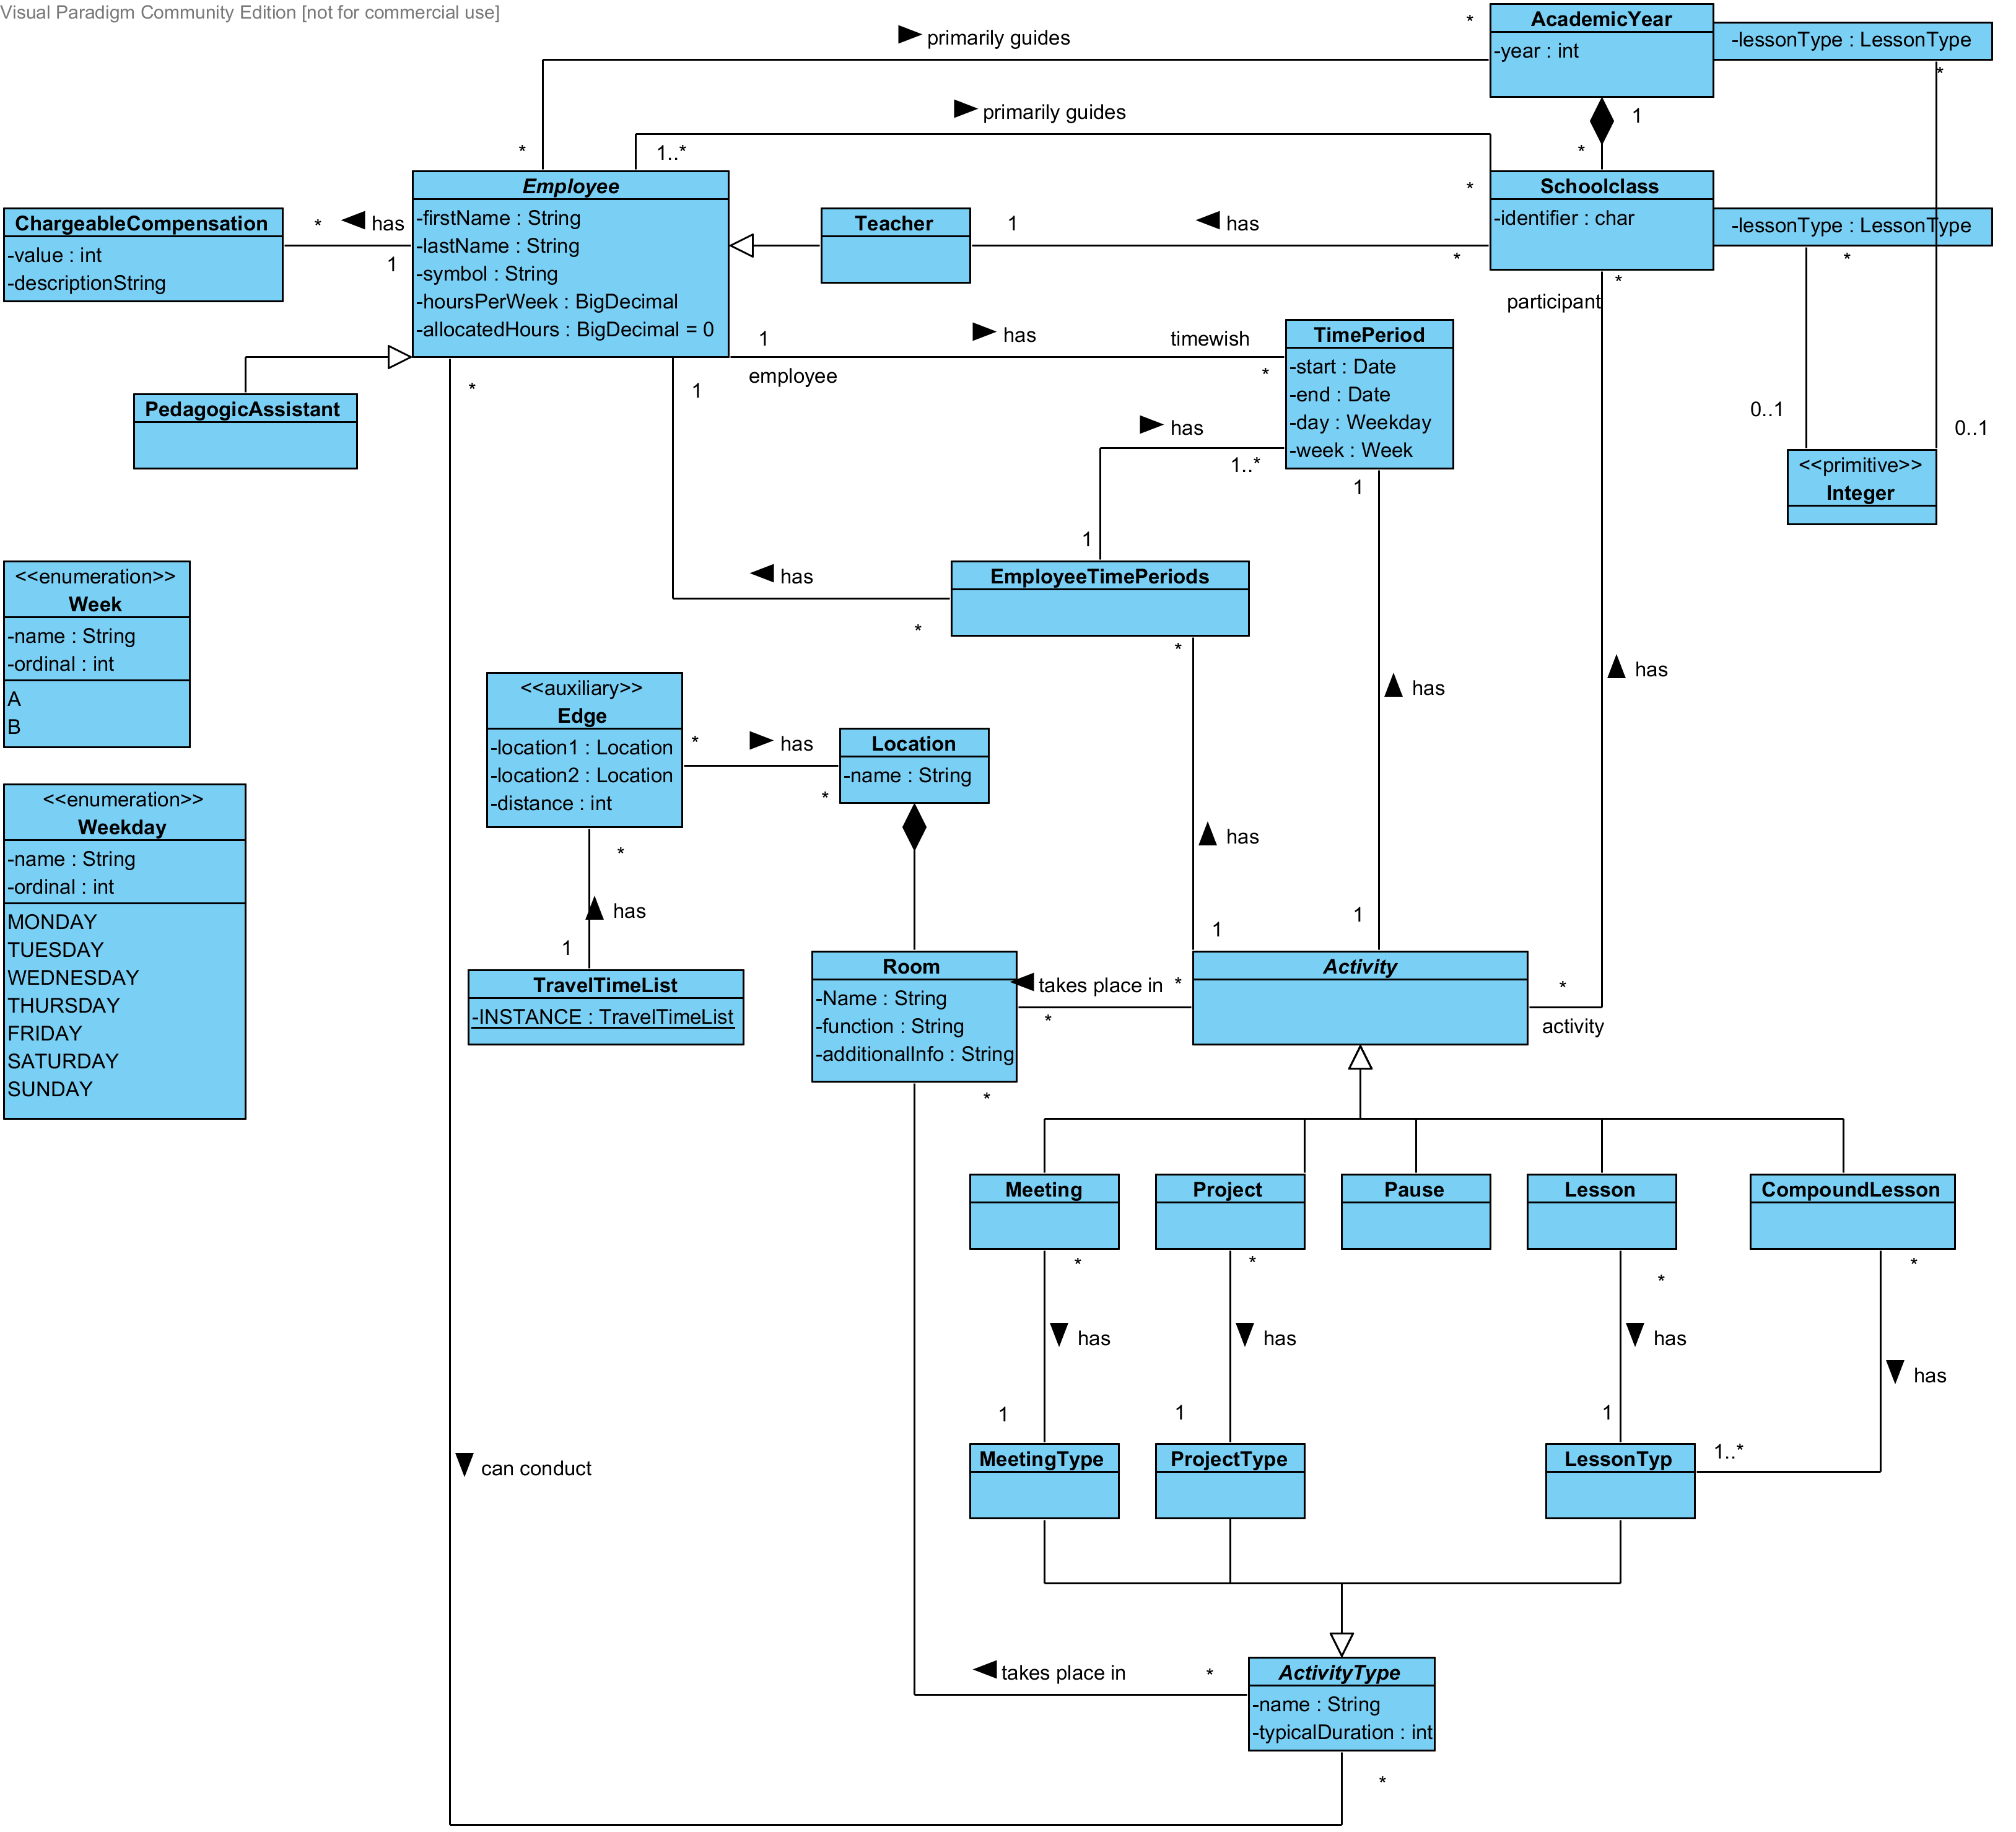
\includegraphics[width=\textwidth]{Datenmodell.png}
\caption{Datenmodell}
\end{figure}
Im Folgenden soll das Datenmodell beschrieben werden.\\

\begin{tabularx}{\textwidth}{|p{0.6cm}|p{5cm}|X|}
\hline
\textbf{Nr.} & \textbf{Assoziation} & \textbf{Beschreibung} \\\hline
1 	& \textit{Employee} -- ChargeableCompensation	& Ein Mitarbeiter kann eine beliebige Anzahl
	an anrechenbaren Ersatzleistungen besitzen. Eine spezifische anrechenbare Ersatzleistung ist immer nur einem Mitarbeiter zugeordnet. \\\hline
2	& \textit{Employee} -- AcademicYear 	& Einer belieben Anzahl an Mitarbeitern kann eine 
	beliebige Anzahl an Jahrgängen zugeordnet sein. D.h. ein Mitarbeiter kann auch keinen Jahrgang betreuen und es muss nicht immer ein ganzer Jahrgang von einem Mitarbeiter betreut werden. \\\hline
3	& \textit{Employee} -- Schoolclass		& Von einem bis zu einer beliebigen Anzahl Mitarbeiter 
	ist eine beliebige Anzahl an Klassen zugeordnet. Ein Mitarbeiter muss also nicht zwangsläufig eine Klasse betreuen, aber eine Klasse hat immer mindestens einen Mitarbeiter, der sie betreut.\\\hline
4	& \textit{Employee} -- TimePeriod		& Ein Mitarbeiter hat eine beliebige Menge von 
	Zeiträumen als Zeitwünsche, also als Zeiten zu denen er gerne frei haben möchte. \\\hline
4	& \textit{Employee} -- \textit{ActivityType} & Einer beliebigen Anzahl von Mitarbeitern kann
	eine beliebige Anzahl von Aktivitätstypen als mögliche Stundeninhalte zugeordnet sein. Diese Assoziationen sind also komplett optional. \\\hline
5	& Schoolclass -- LessonType -- Integer \newline
	  AcademicYear -- LessonType -- Integer				& Eine Schulklasse und ein Jahrgang besitzen Unterrichtsbedarfe. Dies wird durch eine Zuordnung von Integer-Werten zu LessonType-Objekten realisiert. Jedes LessonType-Objekt darf in Kombination mit einer Klasse / einem Jahrgang nur einmal vorkommen. \\\hline
6	& Schoolclass -- Teacher 				& Eine beliebige Anzahl an Schulklassen hat genau
	einen Klassenlehrer. Ein Lehrer kann Klassenlehrer mehrere Schulklassen sein. \\\hline
7	& \textit{Activity} -- TimePeriod				& Einer Aktivität steht immer genau ein
	Zeitraum gegenüber.\\\hline
8	& \textit{Activity} -- Room						& Eine Aktivität kann mehreren Räumen
	zugeordnet
	sein.\\\hline
\end{tabularx}

\begin{tabularx}{\textwidth}{|p{0.6cm}|p{5cm}|X|}
\hline
9	& Meeting -- MeetingType 			 & Eine Aktivität vom Typ Meeting hat genau einen
	MeetingType. Ein MeetingType kann mehreren Aktivitäten vom Typ Meeting zugeordnet sein. \\\hline
10	& Project -- ProjectType			& Eine Aktivität vom Typ Project hat genau einen
	ProjectType. Ein ProjectType kann mehreren Aktivitäten vom Typ Project zugeordnet sein. \\\hline
11	& Lesson -- LessonType				& Eine Aktivität vom Typ Lesson hat genau einen
	LessonType. Ein LessonType kann mehreren Aktivitäten vom Typ Lesson zugeordnet sein. \\\hline
12 	& \textit{Activity} -- EmployeeTimePeriods		& An einer Aktivität kann eine beliebige
	Anzahl an Mitarbeitern teilnehmen, da diese früher gehen oder später kommen können, wird jedem Mitarbeiter eine eigene Liste von Zeiträumen zugeordnet. Dies wird durch die Klasse \texttt{EmployeeTimePeriods} realisiert. Einer Aktivität kann eine beliebige Zahl von EmployeeTimePeriods-Objekten zugeordnet sein, aber ein spezifisches EmployeeTimePeriod-Objekt ist immer nur genau einer Aktivität zugeordnet. \\\hline
13 	& EmployeeTimePeriods -- Employee 				& Eine beliebige Anzahl
	EmployeeTimePeriods-Objekte besitzt genau einen Lehrer. Ein Lehrer kann Teil einer beliebigen Anzahl von EmployeeTimePeriods-Objekten sein. \\\hline
14	& EmployeeTimePeriods -- TimePeriod 			& Ein EmployeeTimePeriods-Objekt besitzt
	mindestens eine bis beliebig viele TimePeriod-Objekte. Ein spezifisches TimePeriod-Objekt ist immer nur Teil von genau einem EmployeeTimePeriods-Objekt. \\\hline
15	& \textit{Activity} -- Schoolclass				& Eine beliebige Anzahl von Aktivitäten
	besitzt eine beliebige Anzahl von Schulklassen als Teilnehmer. Schulklassen können die Aktivität nicht
	frühzeitig verlassen, daher gilt für sie der für die Aktivität festgelegte Zeitraum.\\\hline
16	& Location -- Room						& Ein Standort besteht aus beliebig vielen Räumen. 
	Wird der Standort gelöscht, werden auch die Räume gelöscht.\\\hline
17	& \textit{ActivityType} -- Room					& Einer beliebigen Anzahl von Aktivitätstypen
	kann die Ausführung in einer beliebigen Anzahl von Räumen zugeordnet sein. \\\hline
\end{tabularx}

\begin{tabularx}{\textwidth}{|p{0.6cm}|p{5cm}|X|}
\hline
18 	& TravelTimeList -- Edge 					& Ein TravelTimeList-Objekt kann eine beliebige
	Anzahl von Edge-Objekten besitzen. Ein Edge-Objekt kann nur Teil eines TravelTimeList-Objektes sein. \\\hline
19	& Edge -- Location							& Einer beliebigen Anzahl von Edge-Objekten kann 
	eine beliebige Anzahl von Location-Objekten gegenüberstehen. Ein Edge-Objekt hat aber immer zwei disjunkte Location-Objekte.\\\hline 
\end{tabularx}
\subsection{Datentypen und Repräsentation von Multiplizitäten}
\begin{figure}[H]
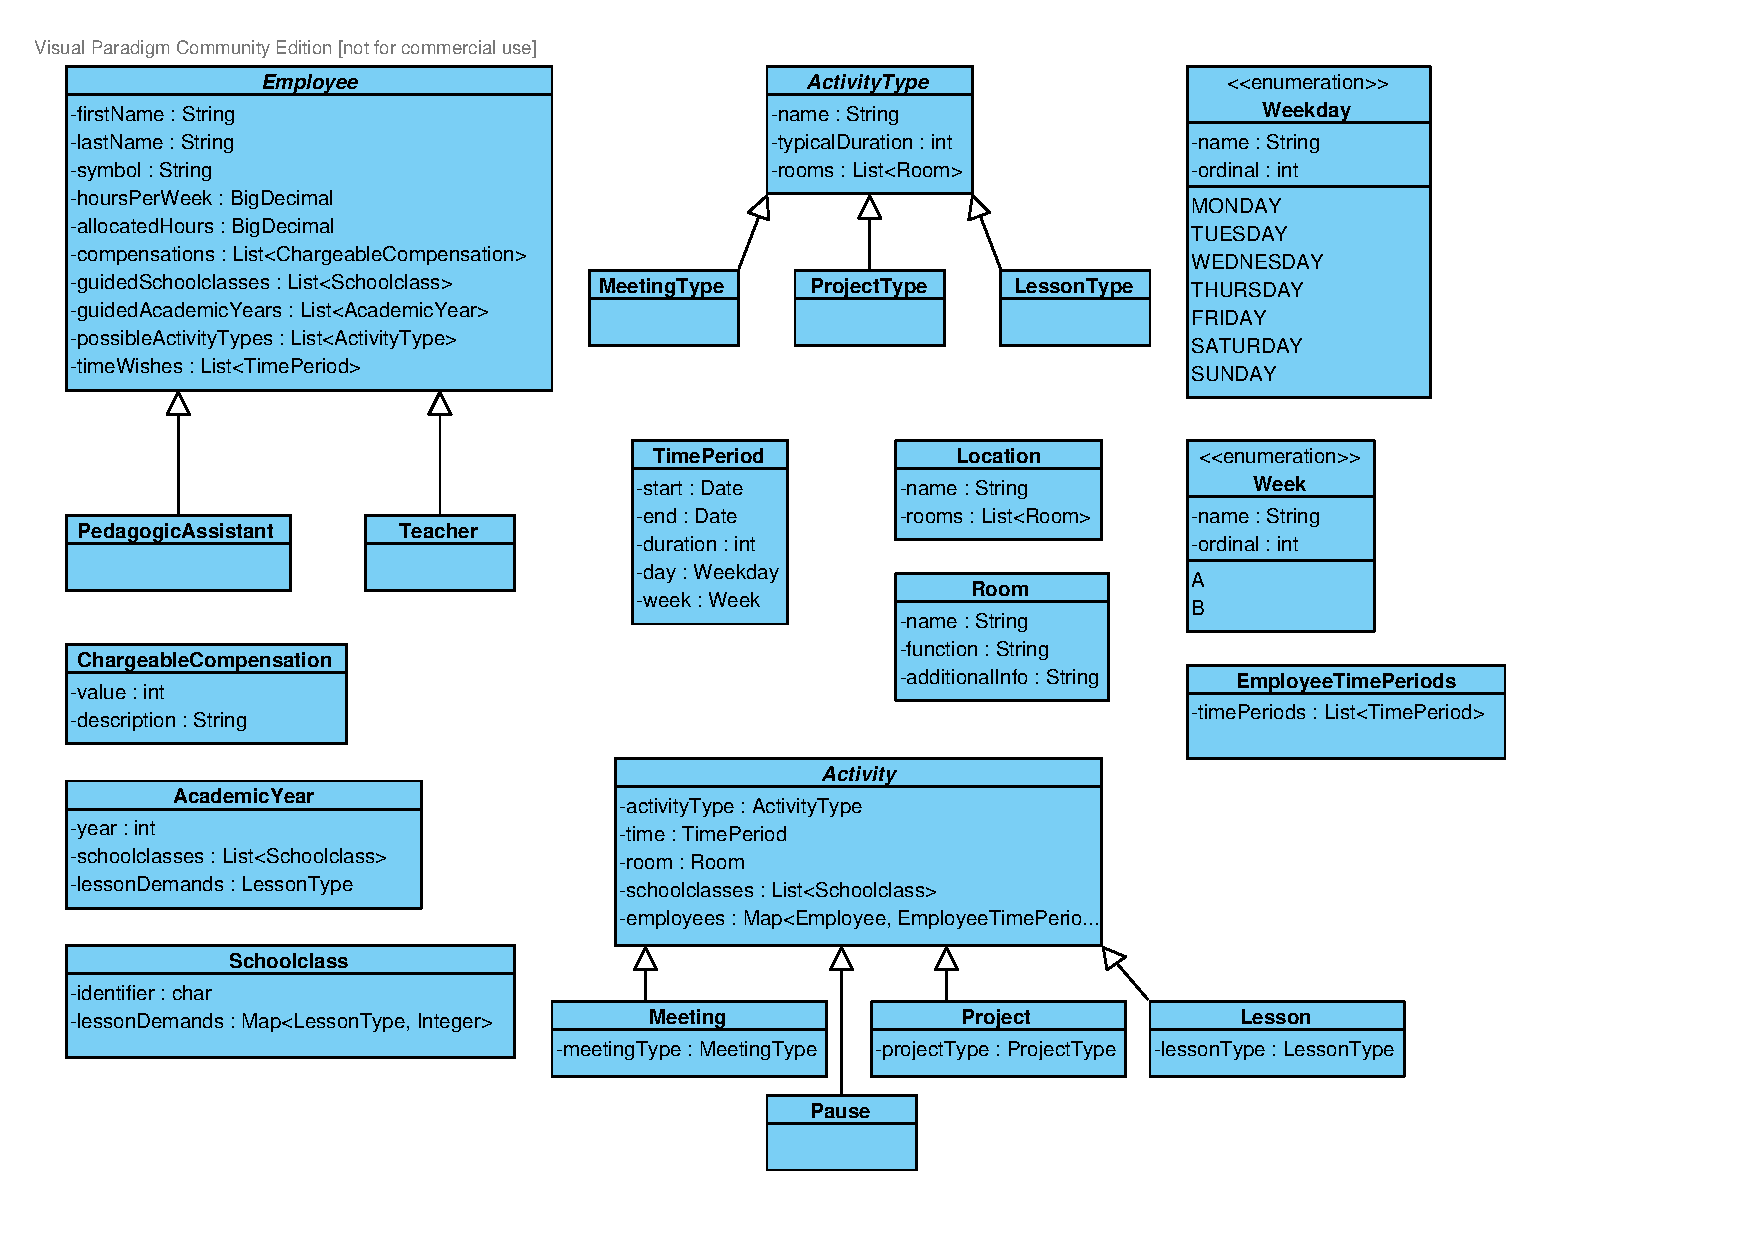
\includegraphics[width=\textwidth]{Datensicht.pdf}
\caption{Übersicht über die Datenklassen}
\end{figure}

Diese Abbildung stellt eine andere Sichtweise auf das Klassendiagramm von Abbildung 3 dar. Es wurden alle Assoziationen weggelassen und dafür die Attribute an die entsprechenden Klassen eingetragen.

\subsection{Abbildung auf die Datenbank}
Die Abbildung auf die Datenbank erfolgt mithilfe des JPA-Frameworks Eclipselink. Es muss lediglich darauf geachtet werden, die Annotationen korrekt zu setzen.  


\section{Ausführungssicht}
\nurlangversion

\label{sec:ausfuehrung}

{\it
Die Ausführungssicht beschreibt das Laufzeitverhalten. Hier
werden die Laufzeitelemente aufgeführt und beschrieben, welche Module
sie zur Ausführung bringen. Ein Modul kann von mehreren
Laufzeitelementen zur Laufzeit verwendet werden. Die Ausführungssicht
beschreibt darüber hinaus, welche Laufzeitelemente spezifisch
miteinander kommunizieren. Zudem wird bei verteilten Systemen
(z.B. Client-Server-Systeme) dargestellt, welche Module von welchen
Prozessen auf welchen Rechnern ausgeführt werden.}


\section[Zusammenhänge zwischen Anwendungsfällen und Architektur]{Zusammenhänge zwischen Anwendungsfällen und Architektur\sectionmark{Zusammenhänge AF u. Architektur}}
\sectionmark{Zusammenhänge AF u. Architektur}
\label{sec:anwendungsfaelle}

{\it In diesem Abschnitt sollen Sequenzdiagramme mit Beschreibung(!)
  für \variante{zwei bis drei von Euch ausgewählte
    Anwendungsfälle}{einen von Euch ausgewählten Anwendungsfall}
  erstellt werden. Ein Sequenzdiagramm beschreibt den
  Nachrichtenverkehr zwischen allen Modulen, die an der Realisierung
  des Anwendungsfalles beteiligt sind.  \variante{Wählt die
    Anwendungsfälle so, dass nach Möglichkeit alle Module Eures
    entworfenen Systems in mindestens einem Sequenzdiagramm
    vorkommen. Falls Euch das nicht gelingt, versucht möglichst viele
    und die wichtigsten Module abzudecken.}{Dazu könnt ihr Euch einen
    Anwendungsfall heraussuchen, der möglichst viele Module der
    Architektur abdeckt. In SWP-2 werden wir mehrere Anwendungsfälle
    betrachten und eine umfangreichere Abdeckung der Architektur
    anstreben.} }

\section{Evolution}
\nurlangversion

\label{sec:evolution}

{\it
  Beschreibt in diesem Abschnitt, welche Änderungen Ihr
  vornehmen müsst, wenn sich Anforderungen oder Rahmenbedingungen
  ändern. Insbesondere sollten hierbei die in der
  Anforderungsspezifikation unter "`Ausblick"' bereits genannten
  Punkte behandelt werden.}

\dots


\end{document} 
